\label{Introduction}
% ---------------------------------------------------
\section{Background}
% \begin{enumerate}
%     \item Ligaments guide and restrict joint motion
%     \item Ligament properties influence knee joint behavior
%     \begin{enumerate}
%         \item Joint mechanics are sensitive to ligament slack length/prestrain
%     \end{enumerate}
%     \item Computer models are used to predict joint behavior
%     \begin{enumerate}
%         \item For intact joints and surgically repaired joints
%         \item Ligament representation varies between models
%     \end{enumerate}
%     \item Regardless of ligament representation, inverse modeling has been used to estimate ligament properties
%     \begin{enumerate}
%         \item Requires two components (1) Experimental testing (2) Joint model
%         \item Simulated experiment is used to iteratively change ligament properties until the computer model's predicted measurements match the experimental measurements
%         \item Ligament properties show large variability between specimens and experiements
%     \end{enumerate}
%     \item Ligament representation varies between models
%     \begin{enumerate}
%         \item Springs have been used to model joint level behavior
%         \item Solid continuum has been used to model joint level behavior as well as specific ligament behavior, however it is computationally expensive, which limits the possibilities for inverse modeling.
%     \end{enumerate}
% \end{enumerate}
%[Ligaments are important to joint function]
%[Computational knee models are used to evaluate different knee treatments and pathology]
Computational joint models are important tools that can be used to better understand joint mechanics and the conditions that can alter joint behavior. Knee models have been used to evaluate joint behavior that is difficult or impossible to measure \textit{in-vitro} or \textit{in-vivo}. Previous studies have used knee models to evaluate the joint's mechanics for healthy \citep{blankevoort_validation_1996,pena_three-dimensional_2006}, injured \citep{ali_validation_2016}, and surgically repaired \citep{thompson_biomechanical_2011,amiri_computational_2012,salehghaffari_phenomenological_2015,smith_influence_2016} joint conditions. Specificmen-specific knee models have been shown to more accurately predict the joint's behavior.

\subsection*{Specimen-Specific Knee Models}
%[The knee model's kinetics and contact mechanics are affected by ligament properties]
Specimen-specific knee models are composed of specimen-specific geometry and material properties. The geometry is normally generated from MR imaging, and material properties for hard and soft tissues are determined with either experimentation \citep{gardiner_subject-specific_2003} or inverse modeling \citep{blankevoort_validation_1996,baldwin_efficient_2009,ewing_estimating_2015,harris_combined_2016}. The joint's kinematics and contact mechanics have been shown to be sensitive to variations in ligament properties under passive \citep{baldwin_efficient_2009,dhaher_effect_2010,ewing_estimating_2015} and dynamic \citep{smith_influence_2016-1} joint loading, therefore specimen-specific ligament properties are needed to model the joint's behavior \citep{ewing_estimating_2015}. In addition to constitutive properties, ligament prestrain must also be defined because each ligament's geometry is defined from MR images, where the ligaments may be under an unknown amount of load \citep{weiss_computational_2001,maas_general_2016}. Specimen-specific prestrain is important to define because joint kinematics have been shown to more sensitive to prestrain than stiffness \citep{baldwin_efficient_2009}. It has been shown that prestrain is not uniform throughout a ligament \citep{hull_strain_1996,gardiner_strain_2001} , and the way that prestrain is applied to a ligament varies depending on the ligament representation.

\subsection*{Ligament Representation and Prestrain Definition}
%[Computational models represent ligaments as nonlinear springs or an anisotropic continuum.]
Ligaments are commonly represented as either bundles of nonlinear uniaxial springs \citep{blankevoort_ligament-bone_1991,baldwin_efficient_2009,amiri_computational_2012,kia_multibody_2016}, or as a solid continuum \citep{gardiner_subject-specific_2003,pena_three-dimensional_2006,dhaher_effect_2010} (\autoref{fig:continuumSpringAcl}). Studies that utilize spring ligament representations can simulate nonhomogeneous prestrain in a ligament by varying the prestrain in each spring that composes a specific ligament. With the exception of \cite{gardiner_subject-specific_2003}, specimen-specific nonhomogeneous prestrain is not utilized in continuum ligament models. Studies that utilize continuum ligament representations either apply uniform prestrain \citep{limbert_three-dimensional_2004,song_three-dimensional_2004,beidokhti_influence_2017}, or nonhomogeneous prestrain based on values reported in the literature \citep{pena_three-dimensional_2006,dhaher_effect_2010}, where prestrains are derived from a combination of experimental studies and results of inverse modeling studies that utilize spring ligament models.

\begin{figure}
    \centering
    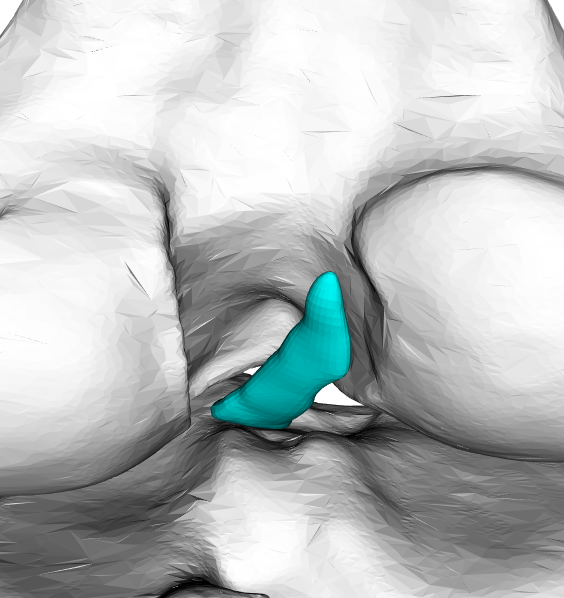
\includegraphics[width=0.35\linewidth]{../img/Knee_ACL_Close.png}
    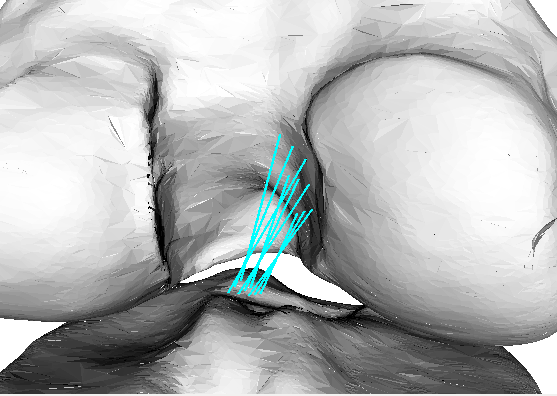
\includegraphics[width=0.45\linewidth]{../img/Knee_ACL_Springs_Close.png}
    \caption{A comparison of the anterior cruciate ligament (ACL) modeled as a (left) continuum and (right) a bundle of nine individual springs arranged across the ligament's insertion site.}
    \label{fig:continuumSpringAcl}
\end{figure}

There are few studies that evaluate the effects of ligament representation on the model's performance, and improvements can be made to the studies that have addressed this topic. \cite{beidokhti_influence_2017} used inverse modeling to generate comparable spring and continuum ligament models. The two types of models were considered equivalent if they yielded joint forces that were similar to experimentally measured values, however it was not shown that the spring and continuum ligament models yielded similar ligament forces at at a given joint position. Additionally, the prestrain definition may not be equivalent between the spring and continuum ligament representations. Conversely, \cite{orozco_effect_2018} applied similar prestrain to their spring and continuum ligament models, however prestrain was uniformly applied throughout each ligament.

% %[Prestrain can be assigned uniformly or nonuniformly across a continuum or spring model. Nonuniform continuum models assign prestrain directly from experimental data, where spring models have estimated prestrain with an inverse modeling scheme.] 
% Nonhomogeneous prestrain can be assigned to spring and continuum ligament representations. Inverse modeling has been used to estimate specimen-specific ligament properties (including nonhomogeneous prestrain) for knee models that represent ligaments as springs \citep{blankevoort_validation_1996,baldwin_efficient_2009,ewing_estimating_2015,harris_combined_2016}. With the exception of \cite{gardiner_subject-specific_2003}, specimen-specific nonhomogeneous prestrain is not utilized in continuum ligament models. Literature is used to define prestrain values \citep{pena_three-dimensional_2006,dhaher_effect_2010}, which are derived from a combination of experimental studies and results of inverse modeling studies that utilize spring ligament models.

% %[Prestrain in a continuum model could be informed with a corresponding calibrated spring model.]
% A calibrated knee model that represents ligaments as springs could be used to estimate specimen-specific nonhomogeneous prestrain in continuum representations of ligaments. \cite{lu_computational_2007} estimated the prestrain in blood vessels using an inverse elastostatics approach, where the deformed state of the geometry and forces were known, and the stress-free shape of the geometry was estimated.
% \subsection*{Nonhomogeneous Prestrain}
%[Nonhomogeneous prestrain has been estimated using two approaches]

% ---------------------------------------------------
\section{Overview}
%[Research questions and objectices: The purpose of this work is to develop an approach to defining ligament prestrain in a continuum ligament model.] 
A calibrated knee model that represents ligaments as springs could be used to estimate specimen-specific nonhomogeneous prestrain in continuum representations of ligaments. \cite{lu_computational_2007} estimated the prestrain in blood vessels using an inverse elastostatics approach, where the deformed state of the geometry and forces were known, and the stress-free shape of the geometry was estimated. The overall purpose of this work is to (1) develop an approach to estimating specimen-specific nonhomogeneous prestrain in ligaments that are represented as a continuum and (2) compare the performance of the continuum ligament representation to an equivalent spring ligament representation.

There are four specific aims that are used to work towards the purpose of this work. The first aim is to collect specimen-specific force-displacement data under novel loading conditions. These data will be used in an inverse modeling scheme to estimate each specimen's ligament slack lengths. Experimental data will be reduced to identify loading conditions that specifically load individual ligaments, and a subset of loading conditions that load all of the modeled ligaments. The results of the other specific aims will be used to support the estimation of subject-specific nonhomogeneous ligament prestrain in ligaments modeled as a continuum. Force results from the specimen-specific forward kinematics model will be used to define boundary conditions for an inverse elastostatics analysis, and the reduced set of loading conditions will be used to evaluate the calibrated continuum ligament models.

This work will develop and evaluate an approach to defining specimen-specific nonhomogeneous prestrain in ligaments modeled as a continuum. This approach could be used improve knee models that are used to evaluate ligament injury, and offer a better comparison between knee models that represent ligaments as springs and a continuum. 

% ---------------------------------------------------
\subsection{Specific Aims}
% ........................
\subsubsection{Experimental Testing}
Experimental testing was conducted to collect specimen-specific force-displacement data and MR images for two specimens. These tests applied novel loading that was designed to remove articular contact which focuses the joint's force-displacement behavior on the soft tissue restraints. The applied joint forces and the corresponding joint kinematics were measured throughout testing. The MR imaging provides the data necessary to create specimen-specific geometry, and the measurements taken during preparation and testing will provide the data necessary to simulate the experimental conditions.

\emph{Status:} Complete

\emph{Contribution:} Data necessary to create specimen-specific models and simulate the experimental tests.
% ........................
\subsubsection{Inverse Modeling}
Inverse modeling was used to estimate specimen-specific ligament slack-lengths. Use of an experimentally novel joint state and joint loads allows for joint contact to be neglected in the computational model, and may focus the joint's force-displacement behavior on the ligaments. Neglecting contact enables the use of a computationally efficient forward kinematics model, which is used in an inverse modeling scheme to estimate ligament slack-length. This will provide a calibrated model that recreates the experimental conditions. 

\emph{Status:} Complete

\emph{Contribution:} A novel approach to using inverse modeling to estimate ligament properties.
% ........................
\subsubsection{Dataset Reduction}
The purpose of this aim is to determine (1) experimental loading conditions that target a small set of ligaments and (2) define a subset of the experimental tests that target all of the modeled ligaments. The experiments applied five different loading conditions at four different flexion angles for a total of twenty tests. Ligament recruitment varies with the loading condition and flexion angle. The specimen-specific geometry and kinematics can be used to estimate ligament length throughout each test, and these length measurements can be used to estimate which ligaments are recruited during specific tests without defining ligament slack lengths.

\emph{Status:} Incomplete

\emph{Contribution:} A set of experimental tests that can be used to evaluate the continuum ligament model's performance.
% ........................
\subsubsection{Continuum Ligament Prestrain}
This aim will use an inverse elastostatic analysis to estimate the undeformed geometry of individual ligaments. To evaluate the performance of this method, experimental

\emph{Status:} Incomplete

\emph{Contribution:} An approach to defining specimen-specific nonhomogeneous prestrain in a continuum ligament model.

% %[Approaches: ]
% \subsection*{Experimental Testing}
% %[Experimental testing focused the joint's force-displacement response on the soft tissue restraints]
% %[Purpose of these tests is to collect force-displacement data under quasistatic loading conditions with forces that do not injure the ligaments.]
% %[Distraction loads were used to isolate the joint's isolate the joint's restraint to the soft tissues.]
% Experimental testing was conducted to collect specimen-specific force-displacement data and MR images for two specimens. These tests applied novel loading that was designed to remove articular contact which focuses the joint's force-displacement behavior on the soft tissue restraints (\autoref{fig:kneeModel}).

% % The MR images were used to generate specimen-specific geometry, including femur and tibia surfaces, and the insertion sites of ligaments (\autoref{fig:kneeModel}). The forward kinematics model was used to simulate experimental tests in an inverse modeling scheme. This scheme used optimization to estimate ligament slack length by minimizing the residual between the calculated and experimentally measured tibial forces. This process is similar to other studies that have used inverse modeling to estimate ligament properties \citep{blankevoort_validation_1996,baldwin_dynamic_2012,ewing_estimating_2015,harris_combined_2016}.
% %Specimen-specific data was collected from experimental laxity-style distraction tests (\autoref{fig:kneeModel}). The experimental data was used to generate a forward kinematics knee model that represented ligaments as springs (\autoref{fig:kneeModel}), and the slack-length for every ligament was estimated using inverse modeling \citep{blankevoort_validation_1996,baldwin_dynamic_2012,ewing_estimating_2015,harris_combined_2016}.

% \begin{figure}
%     \centering
%     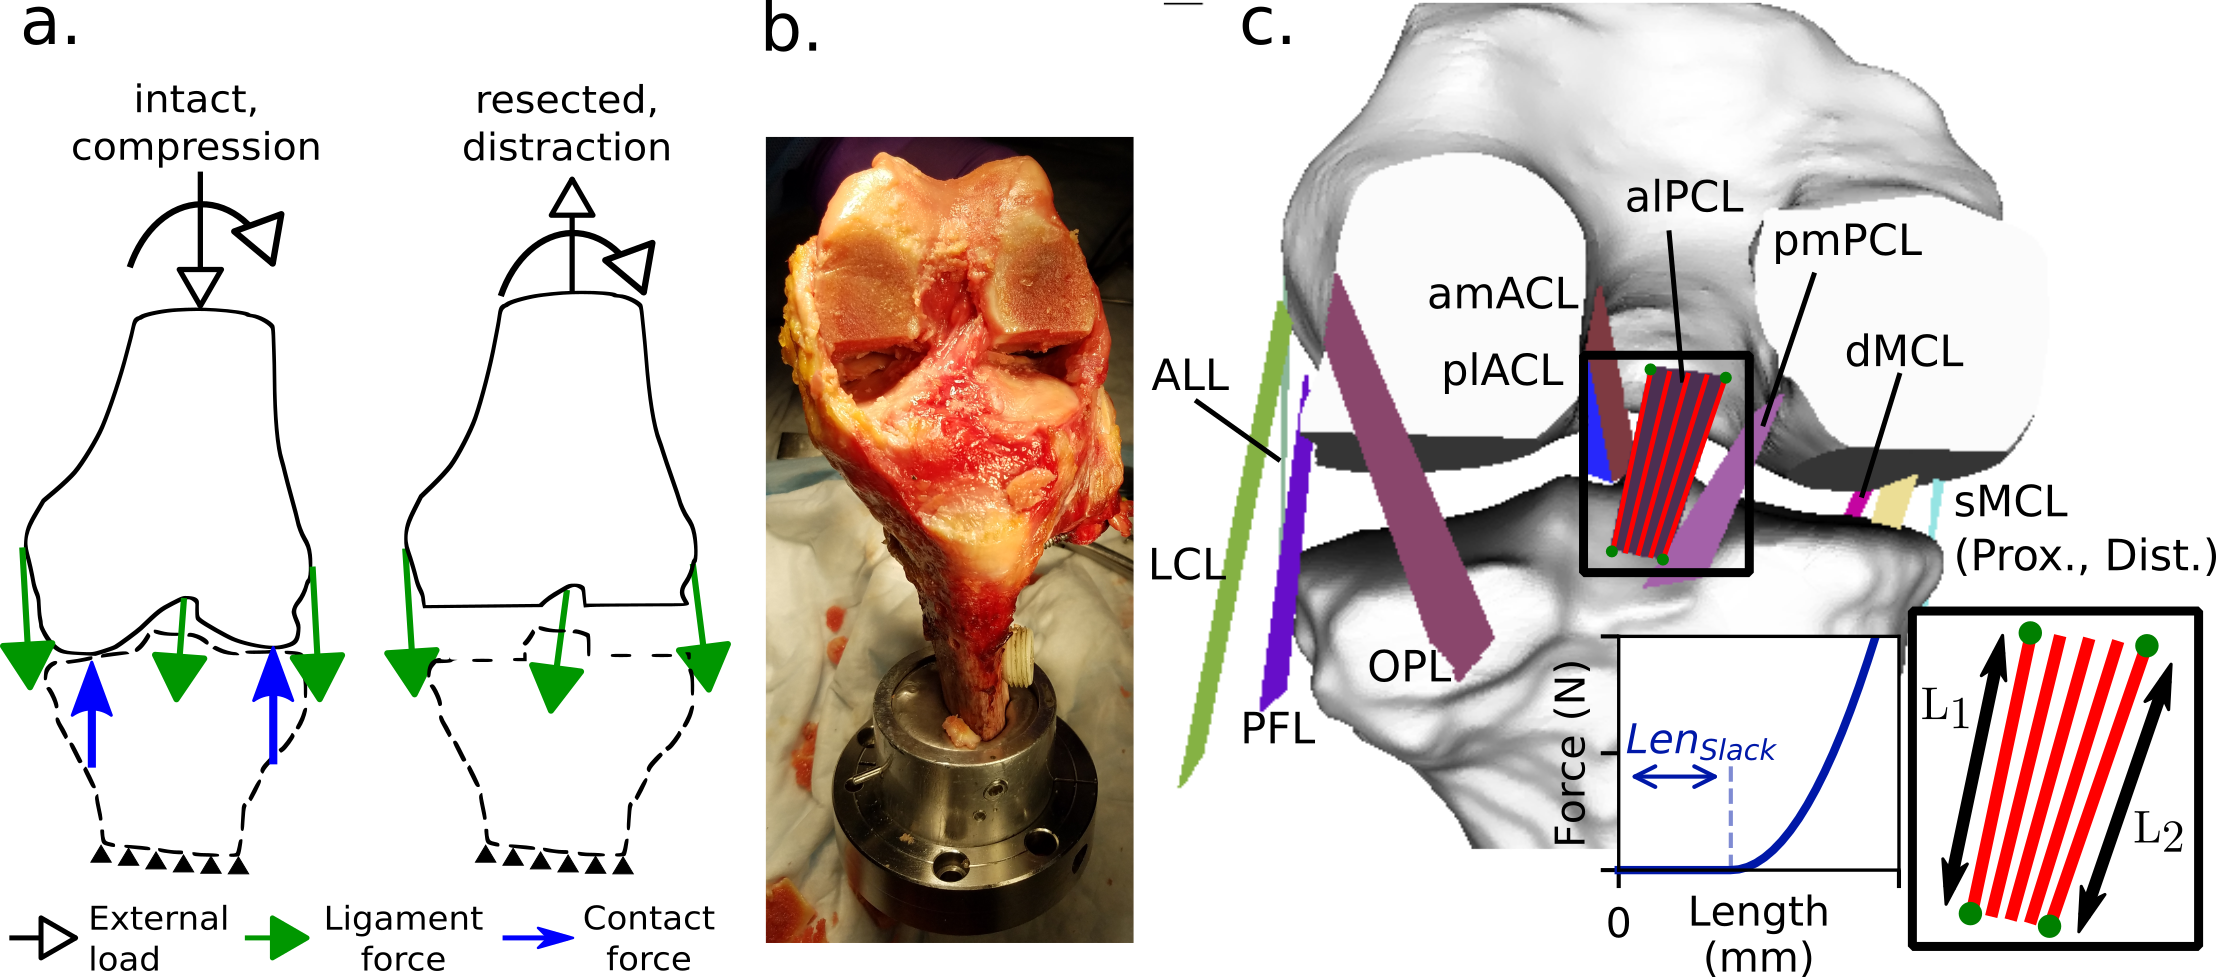
\includegraphics[width=0.85\linewidth]{../img/TwoColumnFig.png}
%     \caption{(a) A similified representation of the joint forces during an intact laxity-style test compared to a distraction laxity-style test. (b) The specimen with resected femoral articulating surfaces. (c) The knee model with 11 ligament bundles represented. (inset) The non-linear spring model, and the definition of slack lenghth for a ligament with five fibers.}
%     \label{fig:kneeModel}
% \end{figure}

% \subsection*{Inverse Modeling}
% %[Specimen-specific slack lengths were estimated using the experimental data and joint geometry in an inverse modeling scheme]
% This approach assumes that the calibrated spring ligament model recreates the ligament's forces at a given joint position. These loading data could be used to define the boundary conditions for a inverse elastostatics analysis of a ligament. \cite{lu_computational_2007} used this approach to estimate the prestrain in blood vessels, where 

% \begin{figure}
%     \centering
%     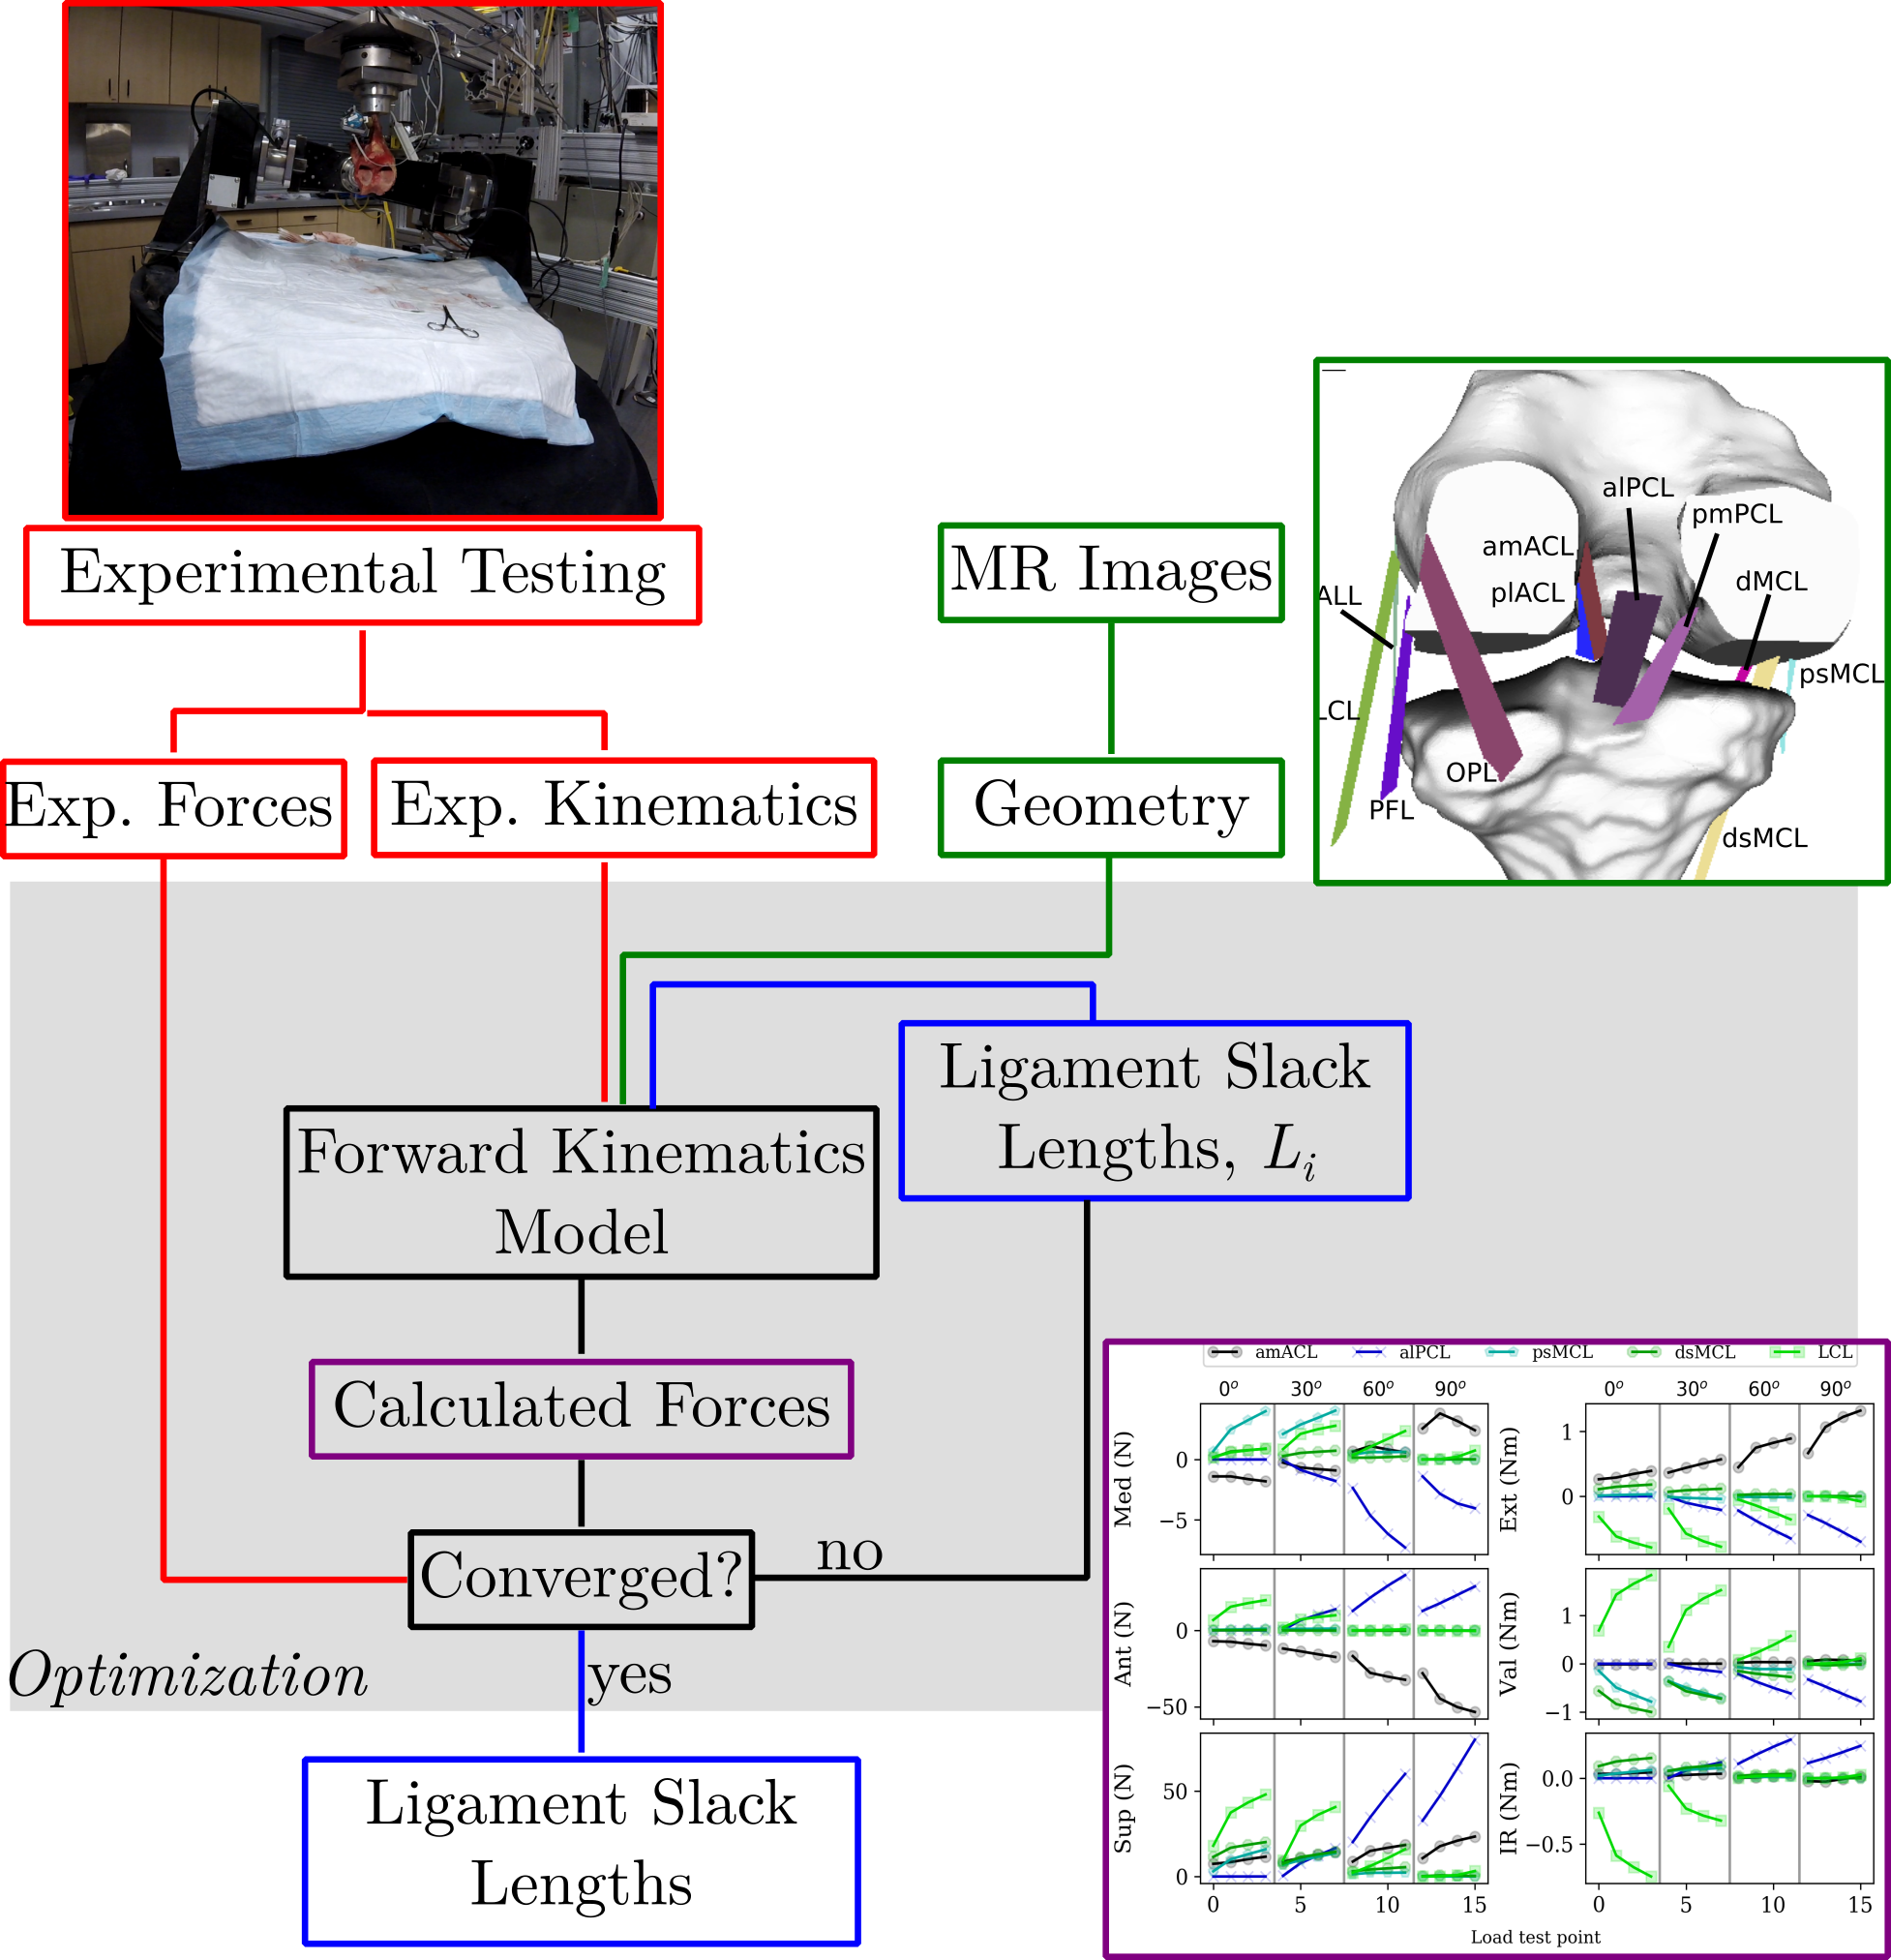
\includegraphics[width=0.95\linewidth]{../img/InverseModelingFlowChart.png}
%     \caption{An overview of how inverse modeling is used to estimate specimen-specific slack lengths. Experimental data is shown with red lines, specimen-specific geometric data is shown with green lines, specimen-specific ligament slack lengths are shown with blue lines, and the purple outlines show the calculated forces for each ligament.}
%     \label{fig:inverseModelingScheme}
% \end{figure}

% \subsection*{Prestrain Estimation}

% \begin{figure}
%     \centering
%     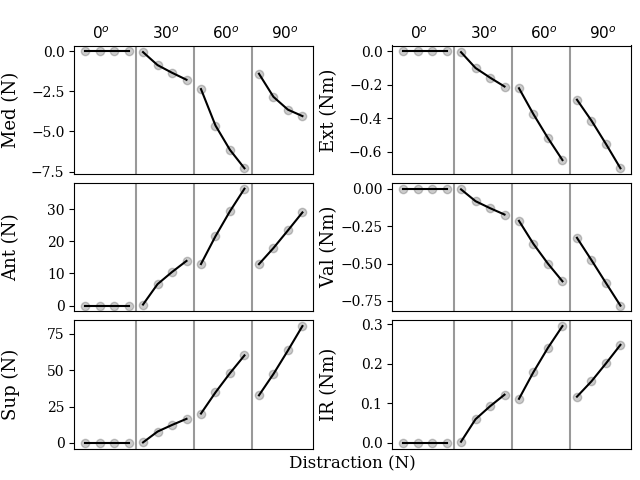
\includegraphics[width=0.75\linewidth]{../img/Spec1_Distraction_alPCL_Forces.png}
%     \caption{An example of the forces and moments that the alPCL exerts on the tibia at four points throughout a distraction test at 0\textsuperscript{o}, 30\textsuperscript{o}, 60\textsuperscript{o}, 90\textsuperscript{o} flexion.}
%     \label{fig:alPclForce}
% \end{figure}

% %[Significance of the work]

% Ligaments are commonly represented as bundles of nonlinear uniaxial springs \citep{blankevoort_validation_1996,baldwin_efficient_2009,ewing_estimating_2015}, or as a solid continuum \citep{gardiner_subject-specific_2003,pena_three-dimensional_2006,dhaher_effect_2010} (\autoref{fig:continuumSpringAcl}). Joint mechanics have been shown to be sensitive to ligament prestrain \citep{baldwin_efficient_2009}, and experimental studies have shown that prestrain is not uniform throughout a ligament \citep{hull_strain_1996,gardiner_strain_2001}. Studies that utilize spring ligament representations can simulate nonhomogeneous prestrain in a ligament by varying the prestrain in each spring that composes a specific ligament. Studies that utilize continuum ligament representations either apply uniform prestrain \citep{limbert_three-dimensional_2004,song_three-dimensional_2004,beidokhti_influence_2017}, or apply nonhomogeneous prestrain based on values reported in the literature \citep{pena_three-dimensional_2006,dhaher_effect_2010}, where prestrains are derived from a combination of experimental studies and results of inverse modeling studies that utilize spring ligament models.

% Representing ligaments as springs allows for the prediction of joint level mechanics such as kinematics \citep{weiss_computational_2001}. Ligaments are normally modeled as bundles of springs, where each spring's insertion lies within the insertion area of the ligament. Nonhomogenous prestrain can be simulated by varying the prestrain assigned to each spring in a ligament. Due to their computational efficiency, spring ligament models are used in inverse modeling studies to estimate ligament properties, including as prestrain \citep{blankevoort_validation_1996,baldwin_dynamic_2012,ewing_estimating_2015,harris_combined_2016}.

% Specimen-specific knee models are defined with geometry derived from MR images, and ligament material properties are normally estimated with inverse modeling \citep{blankevoort_validation_1996,baldwin_dynamic_2012,ewing_estimating_2015,harris_combined_2016}. These models normally utilize spring representations of ligaments because they have been shown to allow for the prediction of joint kinematics \citep{weiss_computational_2001}, and they are computationally efficient. A recent study by \cite{beidokhti_influence_2017} compared the effects of ligament representation on a knee model's predicted joint mechanics. That study used inverse modeling to estimate ligament properties for two different knee models, one with spring ligament representations, and the other with continuum ligament representations. 

% A recent study compared joint mechanics between knees modeled with spring and continuum ligament representations for passive loading \citep{beidokhti_influence_2017}. This study evaluated the effects of ligament representation on joint mechanics, however the prestrain definition between two types of ligament representations may not be equivalent. \cite{beidokhti_influence_2017} used inverse modeling to generate comparable spring and continuum joint level models. Multiple springs were used to model each of the cruciate and collateral ligaments, where each spring can have a unique prestrain. Conversely, each continuum ligament was modeled as one body that had prestrain uniformly applied throughout. \cite{gardiner_subject-specific_2003} showed that an nonhomogenous prestrain can have an impact on the strain distribution within a ligament under load. 

% %[The approach will use inverse modeling to first calibrate a spring model.]

% %[Force results from the spring model will be used as boundary conditions for the]

